\section{Свободное движение}
Рассмотрим систему, заданную дифференциальным уравнением
\begin{equation}
    \ddot{y} + a_1 \dot{y} + a_0 y = u
    \label{eq:system}
\end{equation}
Для построения структурной схемы данной системы перепишем ее в операторном виде и преобразуем выражение: 
\begin{equation}
    p^2 y + a_1 p y + a_0 y = u
\end{equation}
\begin{equation}
    p^2 y = u - a_1 p y - a_0 y
    \notag
\end{equation}
\begin{equation}
    y = \frac{1}{p^2} u - \frac{a_1}{p} y - \frac{a_0}{p^2} y
    \notag
\end{equation}
\begin{equation}
    y = \frac{1}{p^2} \left( u -a_1py - a_0y \right) 
    \notag
\end{equation}
структурная схема приведена на рисунке \ref{fig:scheme1}.
\begin{figure}[ht!]
    \centering
    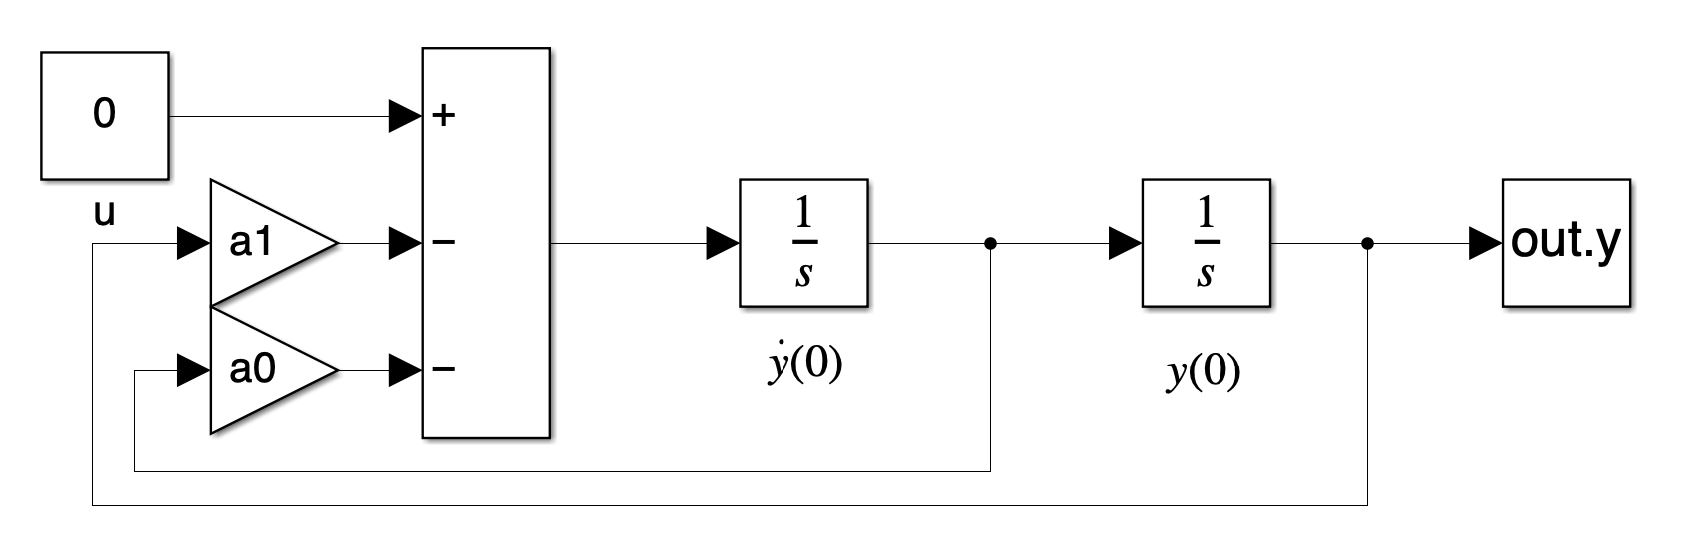
\includegraphics[width=\textwidth]{media/scheme1.png}
    \caption{Структурная схема системы}
    \label{fig:scheme1}
\end{figure}

\subsection{Определение значения коэффициентов}
Так как мы рассматриваем свободное движение, то входное воздействие $u = 0$.

Для определения коэффициентов $a_0$ и $a_1$ из корней характеристического уравнения воспользуемся теоремой Виета:
\begin{equation}
    \lambda^2 + a_1 \lambda + a_0 = 0
    \label{eq:char_eq}
\end{equation}
\begin{equation}
    a_0 = \lambda_1 \lambda_2\quad a_1 = -(\lambda_1 + \lambda_2)
\end{equation}
Составим таблицу с коэффициентами для всех экспериментов:
\begin{table}[ht!]
    \centering
    \begin{tabular}{|c|c|c|c|c|c|c|c|c|}
        \hline
        Номер & $\lambda_1$ & $\lambda_2$ & $y(0)$ & $\dot{y}(0)$ & $a_0$ & $a_1$ & $c_1$ & $c_2$ \\
        \hline
        $1$ & $-5.5$ & $-6$ & $1$ & $0$ & $33$ & $11.5$ & $12$ & $-11$ \\
        \hline
        $2$ & $-2.8 + 6j$ & $-2.8 - 6j$ & $1$ & $0$ & $43.84$ & $5.6$ & $10$ & $0.466$\\
        \hline
        $3$ & $18j$ & $-18j$ & $1$ & $0$ & $324$ & $0$ & $1$ & $0$\\
        \hline
        $4$ & $0.8 + 6j$ & $0.8 - 6j$ & $0.05$ & $0$ & $36.64$ & $-1.6$ & $0.05$ & $-0.00666$ \\
        \hline
        $5$ & $5.5$ & $6$ & $0.05$ & $0$ & $33$ & $-11.5$ & $0.6$ & $-0.55$\\
        \hline
        $6$ & $-1.7$ & $1.7$ & $0$ & $0.1$ & $-2.89$ & $0$ & $-0.029$ & $0.029$\\
        \hline
    \end{tabular}
    \caption{Начальные условия и коэффициенты}
    \label{tab:initial_conditions}
\end{table}


\subsection{Аналитическое решение} 
Для нахождения аналитического решения системы \ref{eq:system} посмотрим на корни характеристического уравнения \ref{eq:char_eq}:
Если оба корня вещественные, то общее решение системы будет иметь вид:
\begin{equation}
    y(t) = c_1 e^{\lambda_1 t} + c_2 e^{\lambda_2 t}
\end{equation}
Если корни комплексно-сопряженные, то общее решение системы будет иметь вид:
\begin{equation}
    y(t) = e^{\alpha t} \left( c_1 \cos(\beta t) + c_2 \sin(\beta t) \right)
\end{equation}
где $c$ -- константы, получаемые из начальных условий путем дифференцирования и подстановки в уравнение. 
И $\alpha$, $\beta$ -- вещественная и мнимая части корней характеристического уравнения.

Рассмотрим нахождение начальных условий для случая с вещественными корнями. 
\begin{equation}
    \dot{y} = \lambda_1 c_1 e^{\lambda_1 t} + \lambda_2 c_2 e^{\lambda_2 t}
\end{equation}
\begin{equation}
    \begin{cases}
        y(0) = c_1 + c_2  \\
        \dot{y}(0) = \lambda_1 c_1 + \lambda_2 c_2  \\
    \end{cases}
\end{equation}

\begin{equation}
    \begin{bmatrix}
        1 & 1 \\
        \lambda_1 & \lambda_2
    \end{bmatrix} \times
    \begin{bmatrix}
        c_1 \\
        c_2
    \end{bmatrix} =
    \begin{bmatrix}
        y(0) \\
        \dot(y)(0)
    \end{bmatrix} 
\end{equation}
\begin{equation}
    \begin{bmatrix}
        c_1 \\
        c_2
    \end{bmatrix} = 
    \begin{bmatrix}
        1 & 1 \\
        \lambda_1 & \lambda_2
    \end{bmatrix}^{-1} \times
    \begin{bmatrix}
        y(0) \\
        \dot{y}(0)
    \end{bmatrix}
\end{equation}

И для случая с комплексными корнями:
\begin{equation}
    \dot{y} = \alpha e^{\alpha t} \left( c_1 \cos(\beta t) + c_2 \sin(\beta t) \right) + \beta e^{\alpha t} \left(-c_1 \sin(\beta t) + c_2 \cos(\beta t) \right)
\end{equation}
\begin{equation}
    \begin{cases}
        y(0) = c_1  \\
        \dot{y}(0) = \alpha c_1 + \beta c_2 \\
    \end{cases}
\end{equation}
\begin{equation}
    \begin{bmatrix}
        1 & 0 \\
        \alpha & \beta
    \end{bmatrix} \times
    \begin{bmatrix}
        c_1 \\
        c_2
    \end{bmatrix} =
    \begin{bmatrix}
        y(0) \\
        \dot(y)(0)
    \end{bmatrix}
\end{equation}
\begin{equation}
    \begin{bmatrix}
        c_1 \\
        c_2
    \end{bmatrix} = 
    \begin{bmatrix}
        1 & 0 \\
        \alpha & \beta
    \end{bmatrix}^{-1} \times
    \begin{bmatrix}
        y(0) \\
        \dot{y}(0)
    \end{bmatrix}
\end{equation}

Посчитанные коэффициенты занесены в таблицу \ref{tab:initial_conditions}.

\subsection{Моделирование}
Выполним моделирование каждого из экспериментов в Matlab. Кроме того, сравним 
результаты моделирования с аналитическим решением. (см. рисунки \ref{fig:case1} -- \ref{fig:case6})

\begin{figure}[hb!]
    \centering
    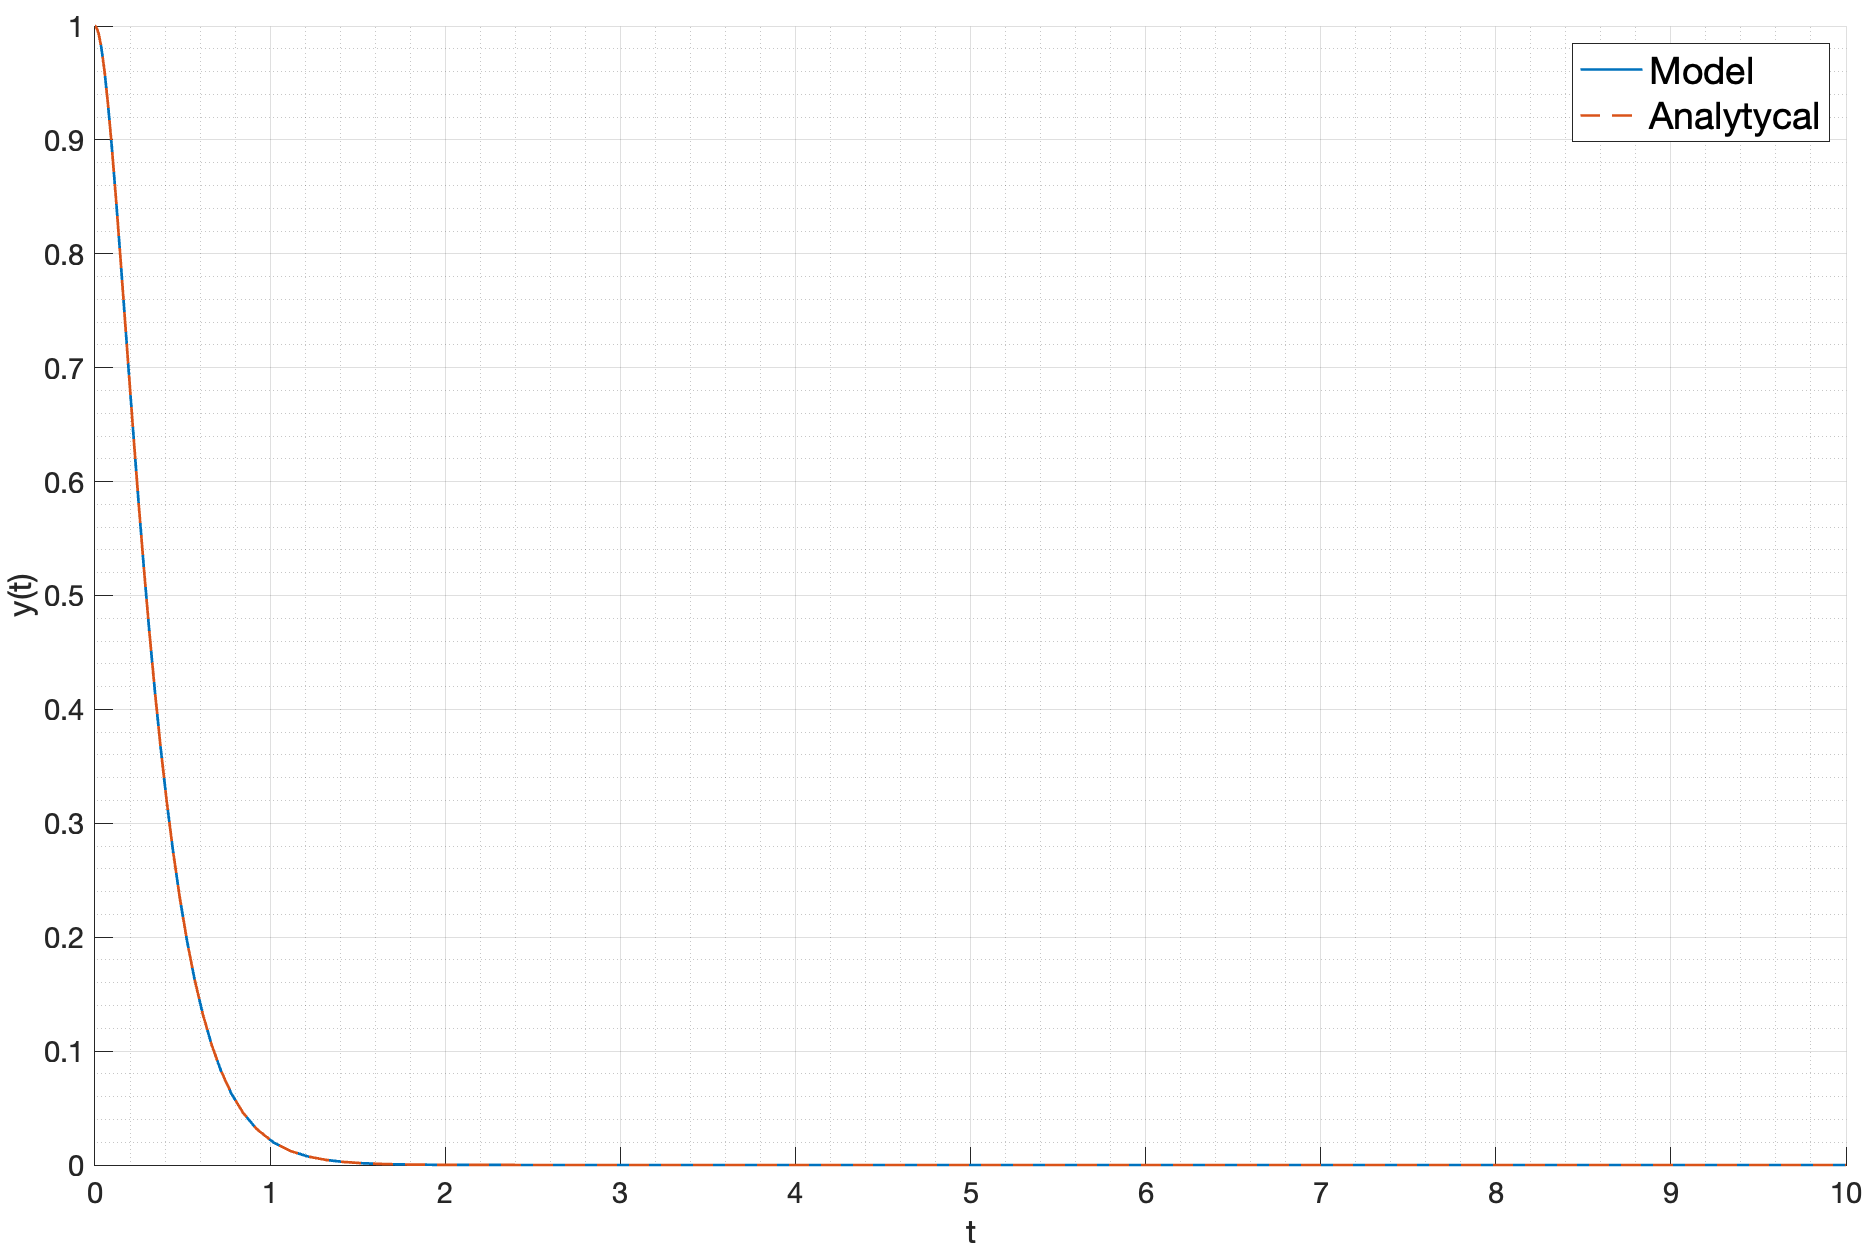
\includegraphics[width=\textwidth]{media/case1.png}
    \caption{График для эксперимента 1}
    \label{fig:case1}
\end{figure}

\begin{figure}[ht!]
    \centering
    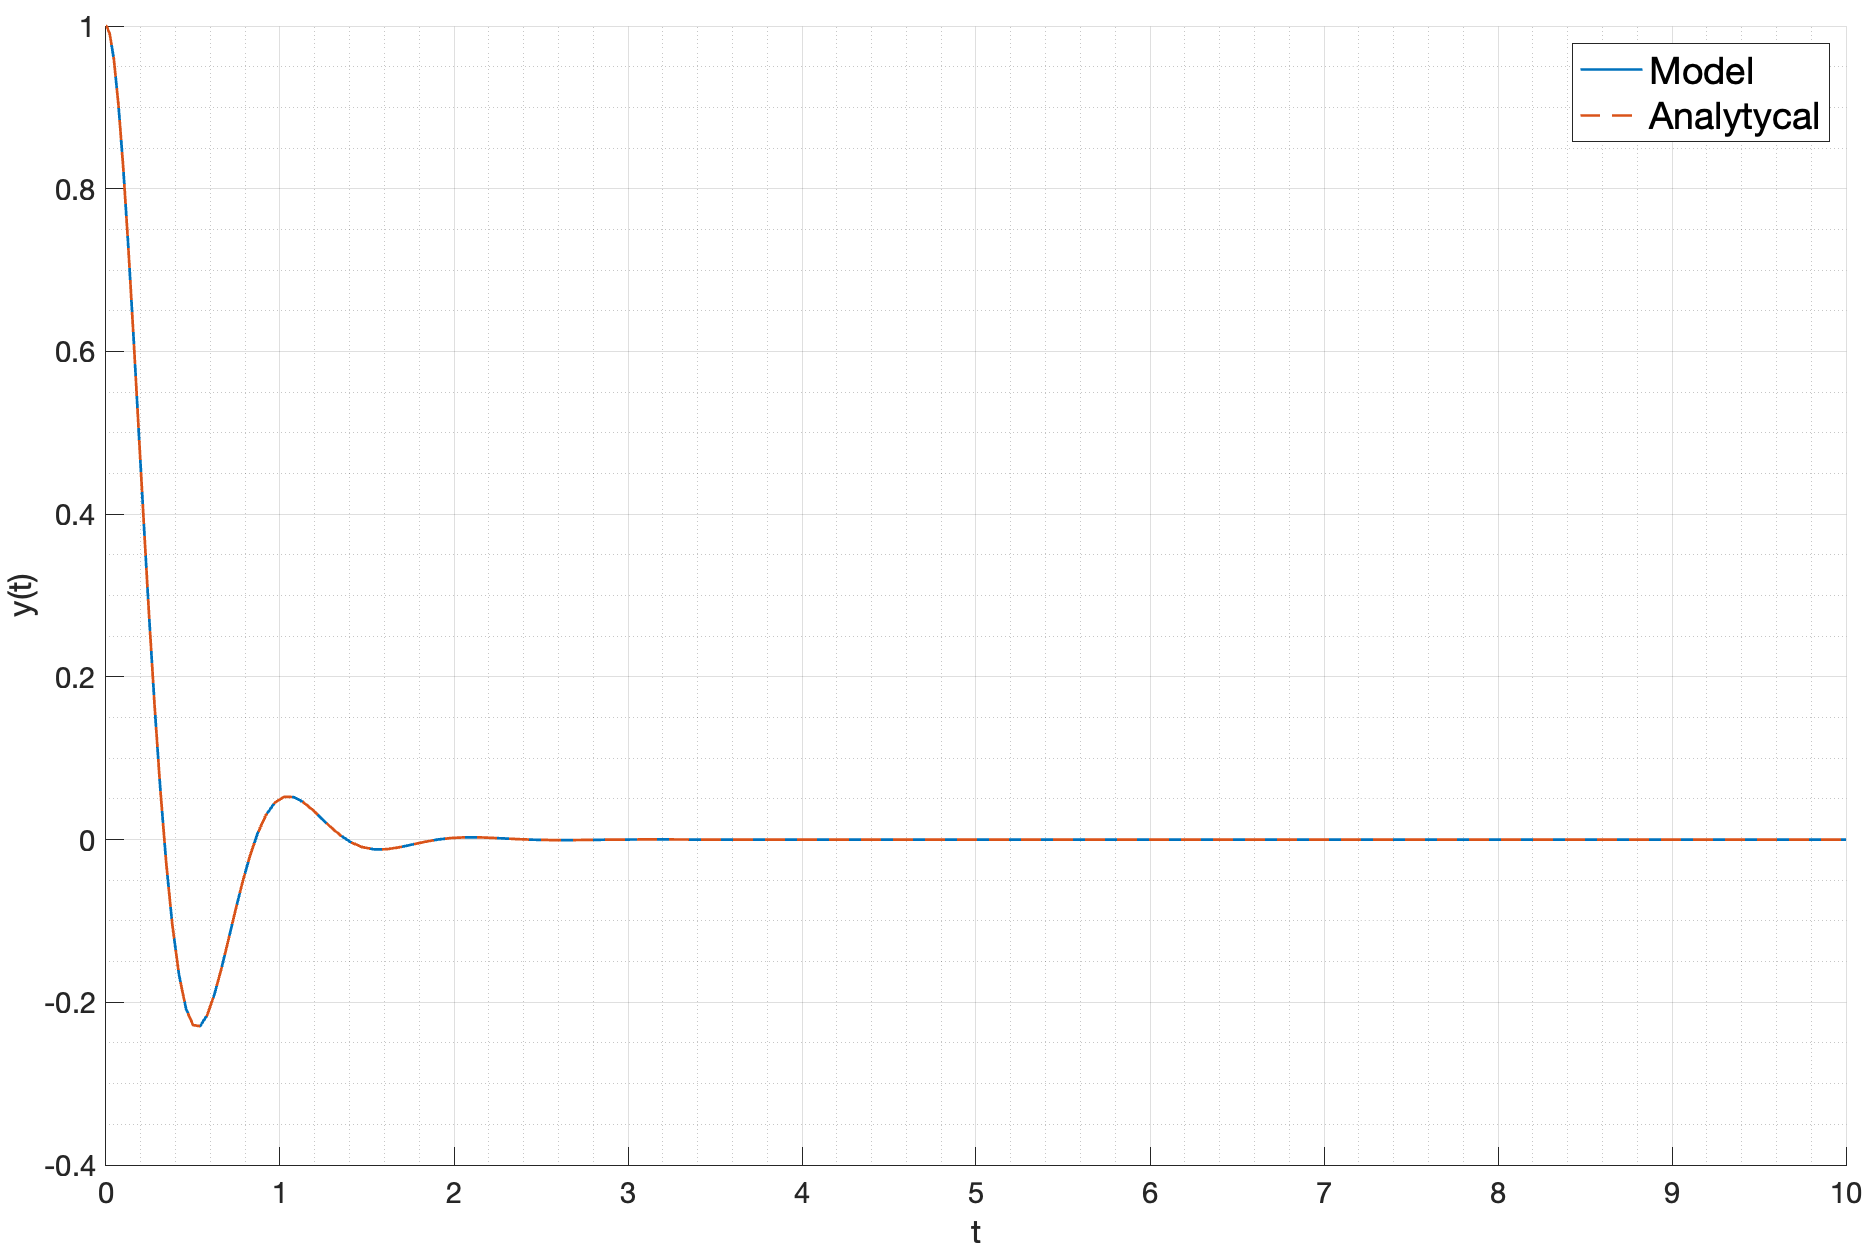
\includegraphics[width=\textwidth]{media/case2.png}
    \caption{График для эксперимента 2}
    \label{fig:case2}
\end{figure}

\begin{figure}[ht!]
    \centering
    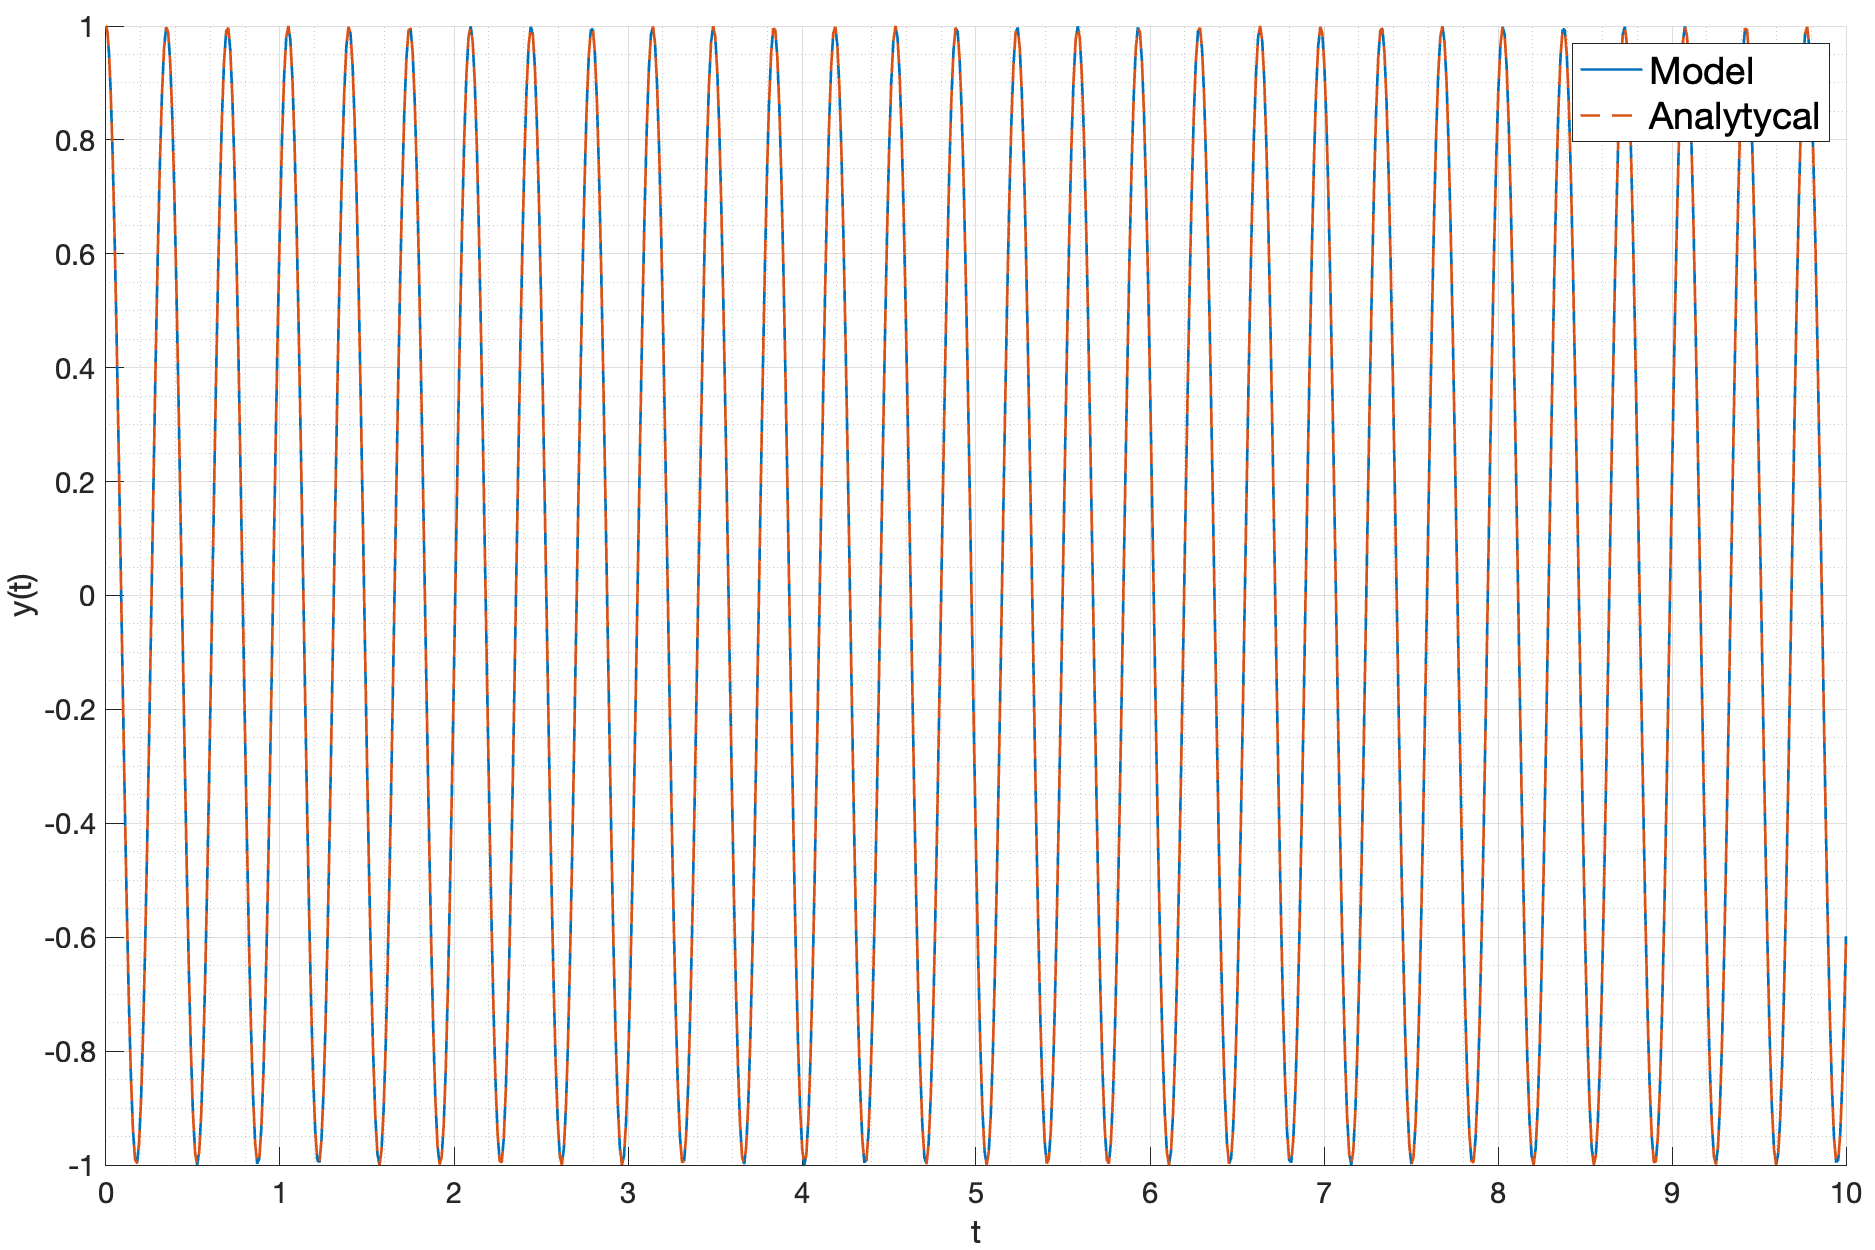
\includegraphics[width=\textwidth]{media/case3.png}
    \caption{График для эксперимента 3}
    \label{fig:case3}
\end{figure}

\begin{figure}[ht!]
    \centering
    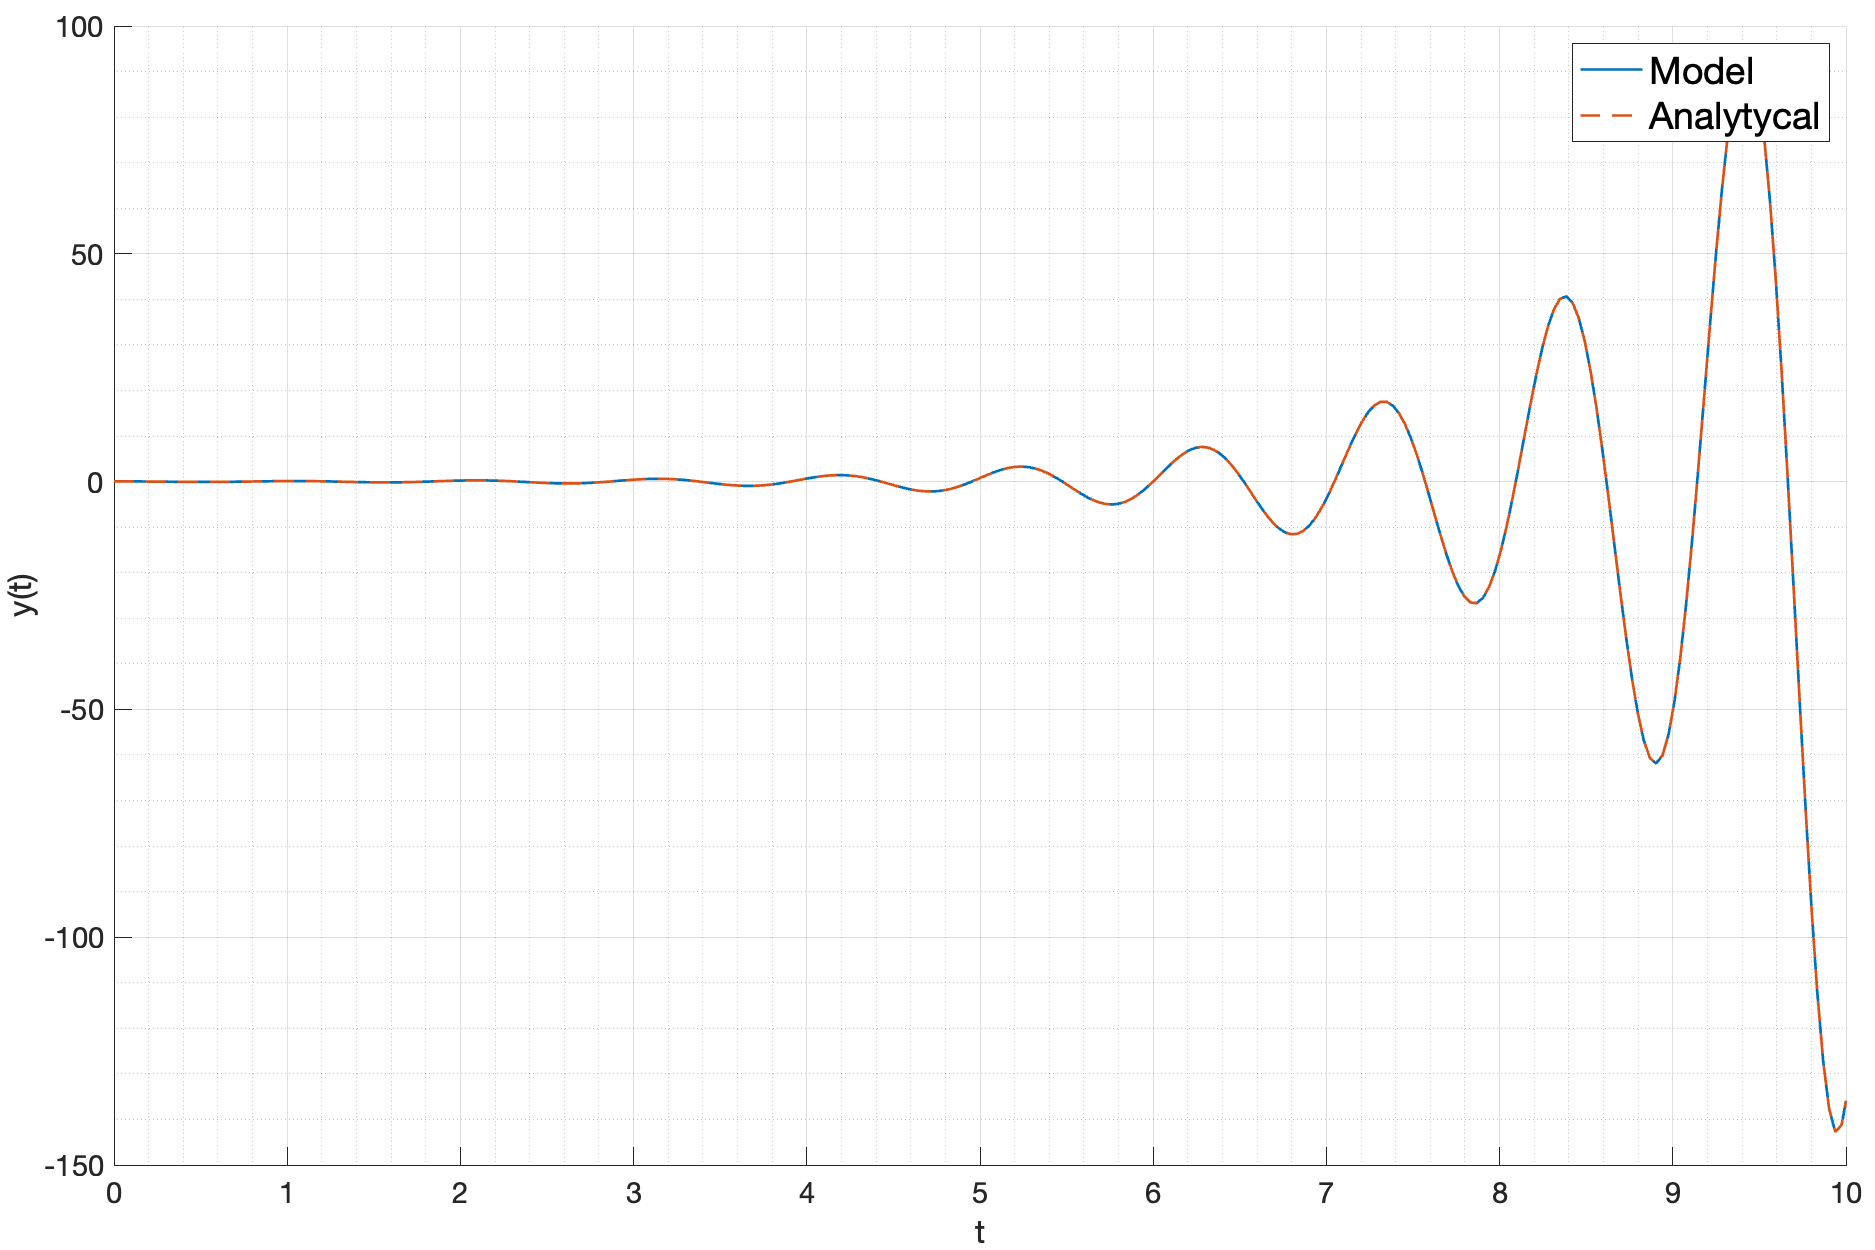
\includegraphics[width=\textwidth]{media/case4.png}
    \caption{График для эксперимента 4}
    \label{fig:case4}
\end{figure}

\begin{figure}[ht!]
    \centering
    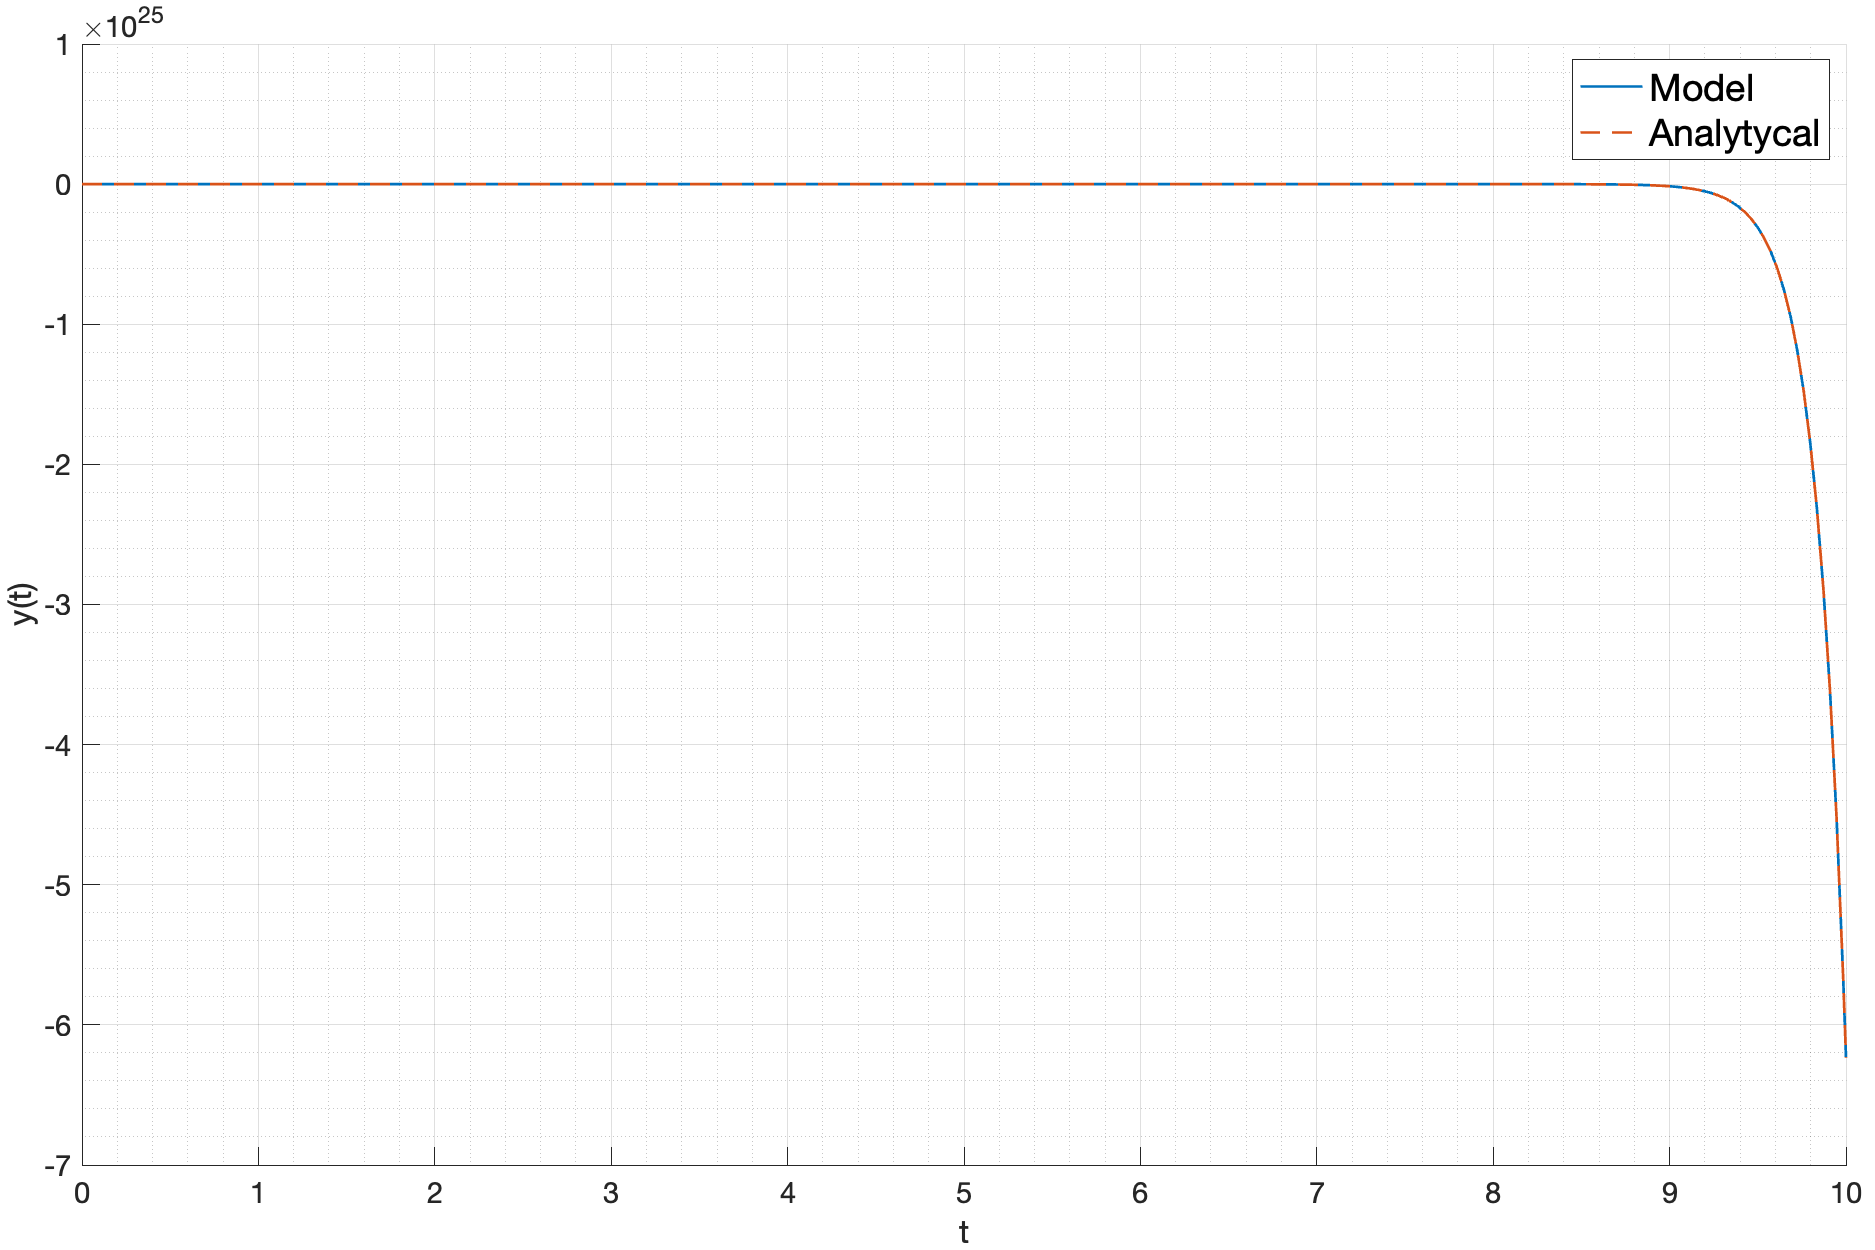
\includegraphics[width=\textwidth]{media/case5.png}
    \caption{График для эксперимента 5}
    \label{fig:case5}
\end{figure}

\begin{figure}[ht!]
    \centering
    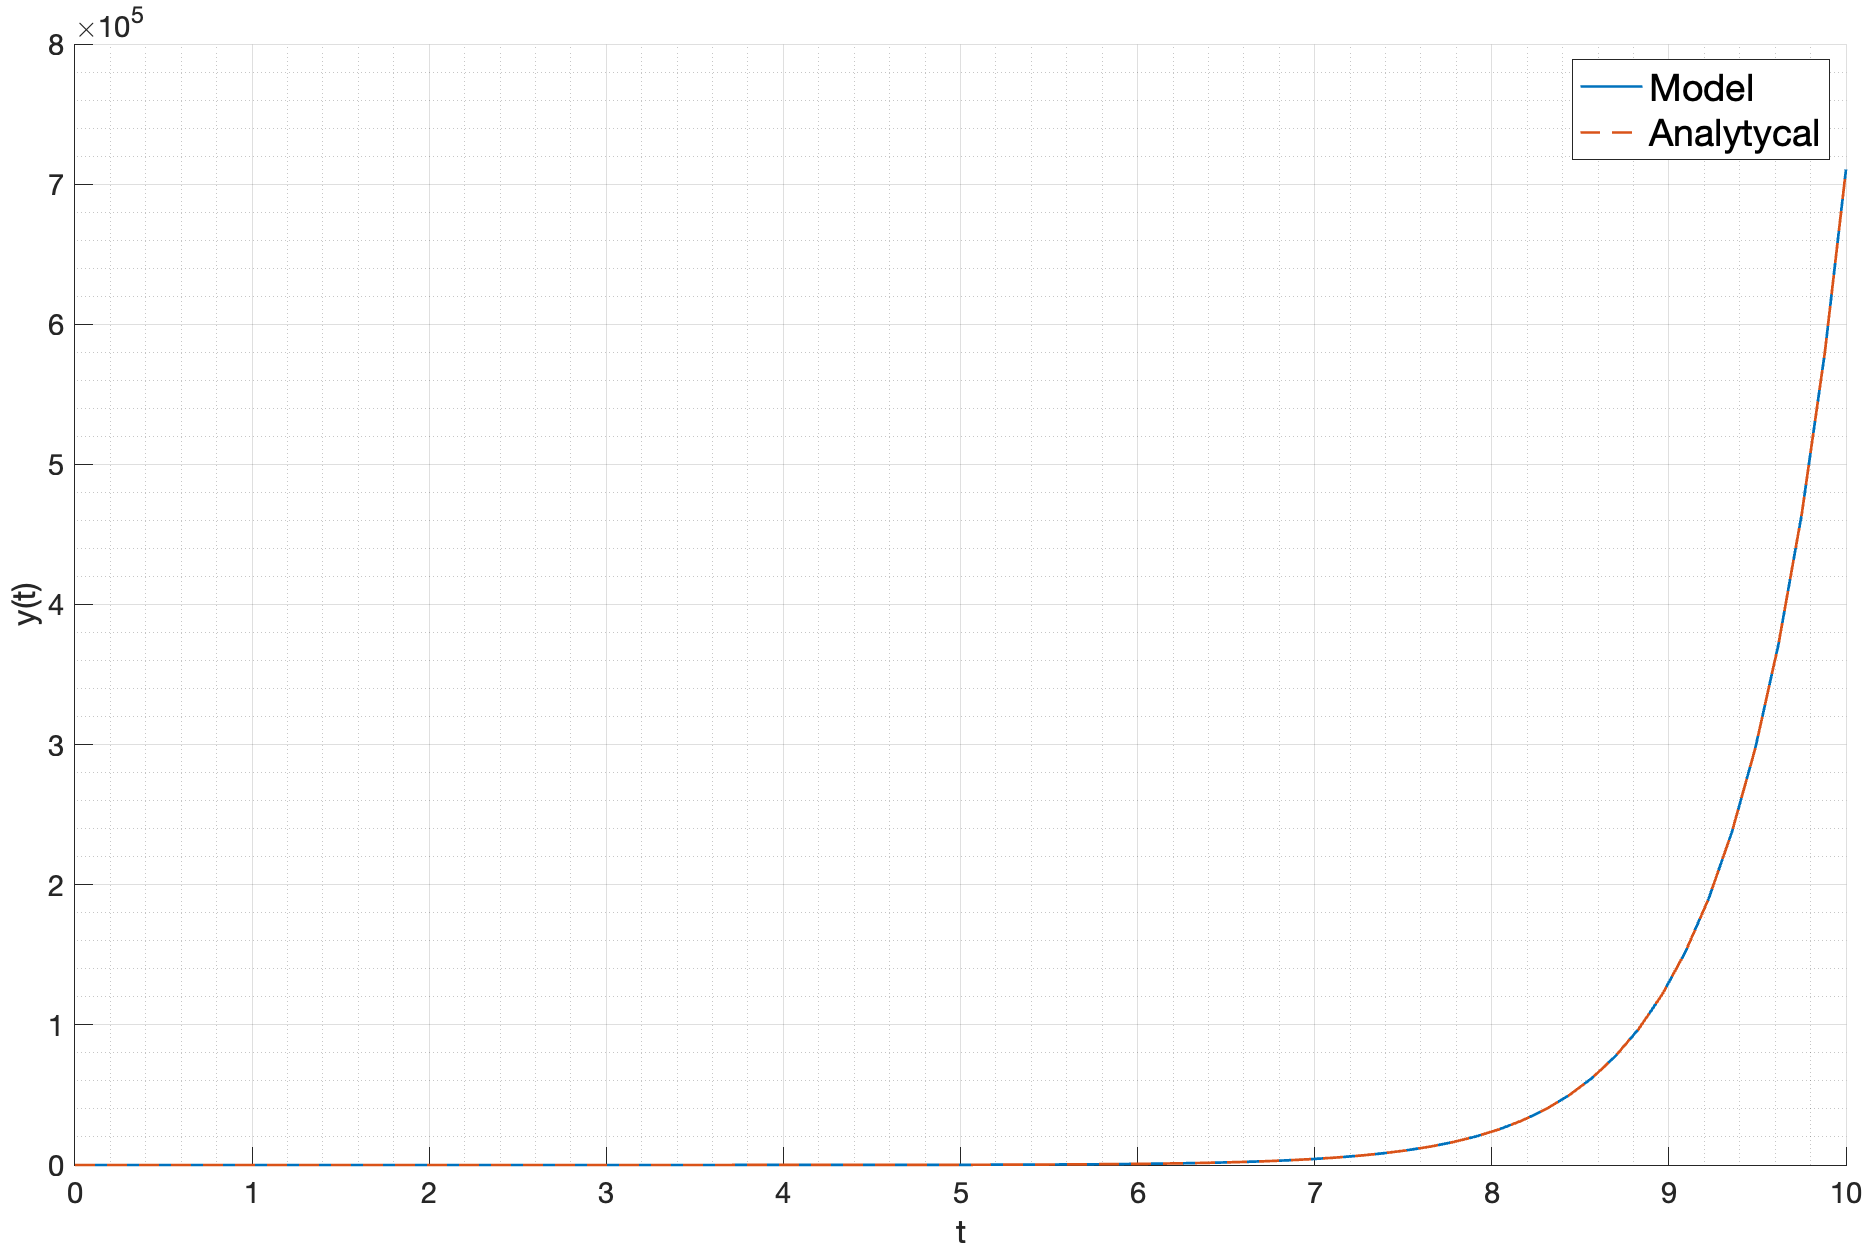
\includegraphics[width=\textwidth]{media/case6.png}
    \caption{График для эксперимента 6}
    \label{fig:case6}
\end{figure}

Видим, что в каждом из случаев моделирование совпадает с аналитическим решением. 
На основании этого можно сделать вывод, что моделирование отражает динамику системы. 

\subsection{Анализ устойчивости систем}

Имея графики для каждого из экспериментов, можно сделать вывод о устойчивости систем. 
Результаты занесены в таблицу \ref{tab:stability}.

\begin{table}[hb!]
    \centering
    \begin{tabular}{|c|c|c|}
        \hline
        Номер & Тип устойчивости & Характер корней\\
        \hline
        $1$ & Устойчива асимптотически & $\forall Re(\lambda) < 0$ \\
        \hline
        $2$ & Устойчива асимптотически  & $\forall Re(\lambda) < 0$ \\
        \hline
        $3$ & Граница устойчивости & $Re(\lambda) = 0,\lambda_1 = \overline{\lambda_2}$ \\
        \hline
        $4$ & Неустойчива & $\exists Re(\lambda) > 0$ \\
        \hline
        $5$ & Неустойчива & $\exists Re(\lambda) > 0$ \\
        \hline
        $6$ & Неустойчива & $\exists Re(\lambda) > 0$ \\
        \hline
    \end{tabular}
    \caption{Устойчивость систем}
    \label{tab:stability}
\end{table}

Для того, чтобы оценить устойчивость систем аналитически, нужно
рассмотреть корни характеристического уравнения.
Если все вещественные части корней характеристического уравнения отрицательны, 
то система устойчива асимптотически. Если все корни отрицательны или нулевые,
при этом нет кратных корней на мнимой оси, то система устойчива по Ляпунову. 
Если есть хотя бы один корень с положительной вещественной частью или кратные 
корни на мнимой оси, то система неустойчива.

\FloatBarrier
\subsection{Выводы}
Мне удалось построить структурную схему системы, решить ее аналитически и
смоделировать в Matlab Simulink для различных начальных условий и корней характеристического уравнения.
Аналитическая оценка устойчивости системы совпала с результатами моделирования. 

